\chapter{Lijndetectie}

\section{Randdetectie}
Randdetectie is het detecteren van randen in een beeld. Vaak wordt dit gerealiseerd door hoge verschillen in pixelintensiteit.
\subsection{Canny randdetector}
Het algoritme verloopt als volgt:
\begin{enumerate}
	\item Er wordt een Gaussische filter met schaal $\sigma$ gedefinieerd.
	\begin{itemize}
		\item Dit is nodig omdat elk beeld wel last heeft van ruis. 
		
		\item Een Gaussische filter van grootte $(2k + 1) \times (2k + 1)$ wordt gedefinieerd als:
		
		$$H_{ij} = \frac{1}{2\pi \sigma^2}\exp\bigg(-\frac{(i - (k + 1))^2 + (j - (k + 1))^2}{2\sigma^2}\bigg) \qquad, 1 \leq i, j \leq 2k + 1$$
		
		\item Voorbeeld van een $5 \times 5$ Gaussische filter met $\sigma = 1.4$:
		
		$$H = \frac{1}{159}\begin{pmatrix}
		2 & 4 & 5 & 4 & 2 \\
		4 & 9 & 12 & 9 & 4 \\
		5 & 12 & 15 & 12 & 5 \\
		4 & 9 & 12 & 9 & 4 \\
		2 & 4 & 5 & 4 & 2
		\end{pmatrix}$$
		
		
	\end{itemize}
	

	\item De Sobel operator wordt toegepast om de gradiënt te vinden.
	\begin{itemize}
		\item Een rand in een beeld kan in meerdere richtingen verschillen. Daarom detecteert het Canny algoritme horizontale, verticale en diagonale randen.
		
		\item De Sobel operator geeft twee matrices met de eerste afgeleide in de horizontale richting $(G_x)$ en verticale richting $(G_y)$.
	
	\end{itemize}
	\item Met deze matrices kan de randsterkte $G$ en richting $\Theta$ gevonden worden.

		\begin{equation*}
			\begin{split}
				& G = \sqrt{G_x^2 + G_y^2} \\
				& \Theta = \arctan 2(G_y, G_x)
			\end{split}
		\end{equation*}

	
	\item Verdun in de richting van de gradiënt.
	\begin{itemize}
		\item Dit zorgt ervoor dat de interessante lijnen terug fijner worden. 
		\item Dit is nodig omdat het originele beeld eerst wazig gemaakt wordt in stap 1.
	\end{itemize}

	\item Thresholding met $T_{strong}$ en $T_{weak}$.
	\begin{itemize}
		\item Pixels met een randsterkte groter dan $T_{strong}$ maken zeker deel uit van een rand.
		\item Pixels met een randsterkte lager dan $T_{weak}$ maken zeker geen deel uit van een rand.
		\item Pixels met een randsterkte groter dan $T_{weak}$ maar kleiner dan $T_{strong}$ maken deel uit van een rand indien ze een buur hebben die ook deel uit maakt van een rand. 
		\item Hoe moeten $T_{strong}$ en $T_{weak}$ gekozen worden?
		\begin{itemize}
			\item De \textbf{methode van Otsu} zoekt de $T_{strong}$ die de intra-klasse variantie minimaliseert:
			
			$$\sigma^2_w(t) = \omega_1(t)\sigma_1^2(t) + \omega_2(t)\sigma_2^2(t)$$
			
			met \begin{itemize}
				\item $\omega_i$ de kans om tot klasse $i$ te behoren.
				\item $\sigma_i$ de standaarddeviatie van klasse $i$.
				\item $t$ de threshold.
			\end{itemize}
			\item $T_{weak}$ wordt dan gelijkgesteld aan de helft van $T_{strong}$.
		\end{itemize}
	\end{itemize}
\end{enumerate}

\section{Lijngroepering}
De vergelijking van een lijn dat door twee punten $(x_1, y_1)$ en $(x_2, y_2)$ gaat:

$$\frac{y - y_1}{y_2 - y_1} = \frac{x - x_1}{x_2 - x_1}$$

of

$$(y - y_1)(x_2 - x_1) = (x - x_1)(y_2 - y_1)$$

\section{Hough transformatie}

\section{Radon transformatie}

\section{Random Sample Consensus (RANSAC)}
Het \textbf{RANSAC} algoritme wordt gebruikt om inliers te zoeken. Vaak wordt het gevolgd door least-mean-squares fitting.


Het \textbf{RANSAC} algoritme werkt als volgt:
\begin{enumerate}
	\item Kies een willekeurig paar van punten $p_1$ en $p_2$.
	\item Tel het aantal punten dat binnen een afstand $\delta$ van het lijnstuk $p_1p_2$ ligt. 
	
	De afstand tussen een lijn $ax + by + c = 0$ en een punt $(x_0, y_0)$ wordt gegeven door:
	
	$$\delta = \frac{|ax_0 + by_0 + c|}{\sqrt{a^2 + b^2}}$$
	\item Wanneer het aantal punten een bepaalde threshold overschrijft is de gevonden lijn goed. Anders herstart het algoritme van stap 1.
\end{enumerate} 

Belangrijke parameters zijn:
\begin{itemize}
	\item De afstand $\delta$.
	\item Het aantal punten dat binnen de afstand moeten liggen.
	\item Het aantal pogingen tot dat het algoritme stopt. Aangezien het een random algoritme is bestaat de kans dat het nooit stopt. Daarom is er een stopcriteria nodig.
\end{itemize}

\subsection{Meerdere lijnen}
\begin{figure}[t]
	\centering
	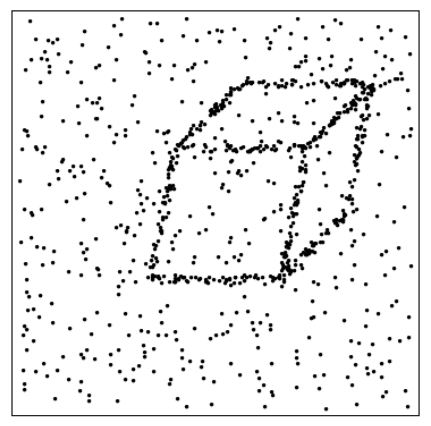
\includegraphics[width=0.7\textwidth]{ransac_multiple_lines}
	\caption{Een afbeelding met 9 lijnen waarbij elke lijn ongeveer 50 punten bevat. In het totaal zijn er 500 punten.}
	\label{fig:ransac_multiple_lines}
\end{figure}

Op figuur \ref{fig:ransac_multiple_lines} wordt een afbeelding getoond waarin de randen van een kubus gedetecteerd zijn. Het algoritme kan eenvoudig uitgebreid worden door elke gevonden lijn te verwijderen zodat deze niet opnieuw kan gevonden worden. 

Hoeveel paren van punten zijn er gemiddeld nodig om de eerste lijn te vinden op figuur \ref{fig:ransac_multiple_lines}?
\begin{itemize}
	\item De kans dat een paar van punten op hetzelfde lijnsegment liggen:
	$$9 \times \frac{50}{950} \times \frac{50}{950} = 0.0249$$
	\item De kans dat een paar waardeloos is, is dan:
	
	$$w = 1 - 0.0249$$
	
	\item Stel $p$ de kans dat na $k$ pogingen er minstens één goed paar gevonden is. Dan is 
	
	$$1 - p = w^k = (1 - 0.0249)^k$$
	
	\item Het logaritme nemen geeft:
	
	$$k = \frac{\log_2(1 - p)}{\log_2(1 - 0.0249)}$$
	
	\item Voor $p = 0.99$ is $ k = \pm 182$. Voor $p = 0.999$ is $k = \pm 273$.
\end{itemize}

\subsection{Optimalisaties}
Voor- en nadelen:
\begin{itemize}
	\good In staat om een goede benadering te geven. 
	\good Weinig geheugen nodig. Enkel de twee gekozen punten moet opgeslagen worden.
	\good Kan ook werken voor cirkels, affiene transformaties, ... 
	\alert De parameters moeten handmatig gekozen worden en is vaak moeilijk te bepalen.
	\alert Er is geen bovengrens voor het aantal iteraties dat nodig zijn om uiteindelijk een resultaat te krijgen?
	\alert Het algoritme vraagt in de praktijk veel meer tijd dan de theoretische tijd.
	\alert Het algoritme is niet-deterministisch. Elke uitvoering van het algoritme levert andere resultaten op.
\end{itemize}

Een aantal optimalisaties:
\begin{itemize}
	\item \textbf{Preventieve :}
	\item \textbf{Lokale optimalisatie:}
	\begin{itemize}
		\item Binnen elke iteratie kunnen lokale optimalisaties uitgevoerd worden op het 'best-so-far' paar.
		\item Na het vinden van een 'best-so-far' paar, kunnen verschillende strategieën toegepast worden:
		\begin{enumerate}
			\item Neem alle punten met een afstand kleiner dan $K\theta$ van de huidige lijn en zoek een nieuwe betere lijn. Blijf dit doen tot dat $K = 1$.
			\item Neem nieuwe paren uit de inliers. \todo{snap ik nie}
			\item Combinatie van de vorige twee strategieën.
		\end{enumerate}
		\item Hoeveel keer is een lokale optimalisatie nodig?
		\begin{itemize}
			\item De kans dat het $k-$de paar het 'best-so-far' is, bedraagt $1/k$. Het gemiddeld aantal 'best-so-far' paren binnen $k$ baren is dan:
			
			$$\sum_{n = 1}^k \frac{1}{n} \leq \int_1^k \frac{1}{x}\;dx + 1 = \log_2 k + 1$$
			\item Lokale optimalisatie is dan $O(\log_2 k)$ maal nodig.
			\good Door het logaritmisch karakter zal het weinig verschil uitmaken op de uitvoeringstijd van het algoritme.
		\end{itemize}
	\end{itemize}
	\item \textbf{Gerichte sampling:}
	\begin{itemize}
		\item Er kan met Hough of Radon kandidaten gevonden worden. 
		\item Met RANSAC worden de kandidaten dan verfijnd.
	\end{itemize}
\end{itemize}


